\documentclass[border=4pt]{standalone}

\usepackage{amsmath}
\usepackage{tikz}
\usepackage{mathdots}
\usepackage{yhmath}
\usepackage{cancel}
\usepackage{color}
\usepackage{siunitx}
\usepackage{array}
\usepackage{multirow}
\usepackage{amssymb}
\usepackage{gensymb}
\usepackage{tabularx}
\usepackage{booktabs}
\usetikzlibrary{fadings}
\usetikzlibrary{patterns}


\begin{document}
 


\tikzset{every picture/.style={line width=0.75pt}} %set default line width to 0.75pt        

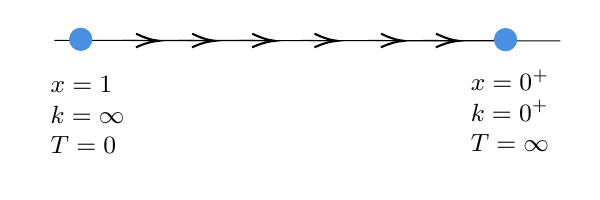
\begin{tikzpicture}[x=0.75pt,y=0.75pt,yscale=-1,xscale=1]
%uncomment if require: \path (0,386); %set diagram left start at 0, and has height of 386

%Straight Lines [id:da08759211767028119] 
\draw    (138,158) -- (381.75,158.25) ;


%Shape: Circle [id:dp5915528169712416] 
\draw  [color={rgb, 255:red, 74; green, 144; blue, 226 }  ,draw opacity=1 ][fill={rgb, 255:red, 74; green, 144; blue, 226 }  ,fill opacity=1 ] (145.33,157.5) .. controls (145.33,154.55) and (147.72,152.17) .. (150.67,152.17) .. controls (153.61,152.17) and (156,154.55) .. (156,157.5) .. controls (156,160.45) and (153.61,162.83) .. (150.67,162.83) .. controls (147.72,162.83) and (145.33,160.45) .. (145.33,157.5) -- cycle ;
%Shape: Circle [id:dp7394374440337268] 
\draw  [color={rgb, 255:red, 74; green, 144; blue, 226 }  ,draw opacity=1 ][fill={rgb, 255:red, 74; green, 144; blue, 226 }  ,fill opacity=1 ] (350,157.67) .. controls (350,154.72) and (352.39,152.33) .. (355.33,152.33) .. controls (358.28,152.33) and (360.67,154.72) .. (360.67,157.67) .. controls (360.67,160.61) and (358.28,163) .. (355.33,163) .. controls (352.39,163) and (350,160.61) .. (350,157.67) -- cycle ;
%Straight Lines [id:da31674232744557984] 
\draw    (171,158) -- (186.25,158.22) ;
\draw [shift={(188.25,158.25)}, rotate = 180.83] [color={rgb, 255:red, 0; green, 0; blue, 0 }  ][line width=0.75]    (10.93,-3.29) .. controls (6.95,-1.4) and (3.31,-0.3) .. (0,0) .. controls (3.31,0.3) and (6.95,1.4) .. (10.93,3.29)   ;

%Straight Lines [id:da9791749441960806] 
\draw    (198,158) -- (213.25,158.22) ;
\draw [shift={(215.25,158.25)}, rotate = 180.83] [color={rgb, 255:red, 0; green, 0; blue, 0 }  ][line width=0.75]    (10.93,-3.29) .. controls (6.95,-1.4) and (3.31,-0.3) .. (0,0) .. controls (3.31,0.3) and (6.95,1.4) .. (10.93,3.29)   ;

%Straight Lines [id:da09075404848094815] 
\draw    (227,158) -- (242.25,158.22) ;
\draw [shift={(244.25,158.25)}, rotate = 180.83] [color={rgb, 255:red, 0; green, 0; blue, 0 }  ][line width=0.75]    (10.93,-3.29) .. controls (6.95,-1.4) and (3.31,-0.3) .. (0,0) .. controls (3.31,0.3) and (6.95,1.4) .. (10.93,3.29)   ;

%Straight Lines [id:da9031512474108416] 
\draw    (257,158) -- (272.25,158.22) ;
\draw [shift={(274.25,158.25)}, rotate = 180.83] [color={rgb, 255:red, 0; green, 0; blue, 0 }  ][line width=0.75]    (10.93,-3.29) .. controls (6.95,-1.4) and (3.31,-0.3) .. (0,0) .. controls (3.31,0.3) and (6.95,1.4) .. (10.93,3.29)   ;

%Straight Lines [id:da5971635597856639] 
\draw    (289,158) -- (304.25,158.22) ;
\draw [shift={(306.25,158.25)}, rotate = 180.83] [color={rgb, 255:red, 0; green, 0; blue, 0 }  ][line width=0.75]    (10.93,-3.29) .. controls (6.95,-1.4) and (3.31,-0.3) .. (0,0) .. controls (3.31,0.3) and (6.95,1.4) .. (10.93,3.29)   ;

%Straight Lines [id:da31869685522957636] 
\draw    (315.5,158) -- (330.75,158.22) ;
\draw [shift={(332.75,158.25)}, rotate = 180.83] [color={rgb, 255:red, 0; green, 0; blue, 0 }  ][line width=0.75]    (10.93,-3.29) .. controls (6.95,-1.4) and (3.31,-0.3) .. (0,0) .. controls (3.31,0.3) and (6.95,1.4) .. (10.93,3.29)   ;


% Text Node
\draw (154,195) node  [font=\small]  {$ \begin{array}{l}
x=1\\
k=\infty \\
T=0
\end{array}$};
% Text Node
\draw (357.5,194) node  [font=\small]  {$ \begin{array}{l}
x=0^{+}\\
k=0^{+}\\
T=\infty 
\end{array}$};


\end{tikzpicture}


\end{document}
